\mysection{Alexander Scheurer}{Logische Übersetzung} \label{sec:logi}

Neben der rein programmatischen Übersetzung der Blender API nach \CS muss auch für Uniplug eine eigene API Struktur geschaffen werden gegen die zukünftige Benutzer von Uniplug bzw. Plugin-Entwickler, programmieren sollen. Diese Struktur muss allgemein gehalten werden damit sie auch die Anbindung weiterer 3D-Softwareprodukte erlaubt. Da die Forschungsgruppe im technischen Bereich eine vollständige Übersetzung der Blender API anstrebt muss auch hier eine ebenso vollständige Lösung gefunden werden. Eine vollständige Lösung bedeutet das nicht nur der Umgang mit 3D-Modellen erreicht werden soll, sondern auch einzele Dreiecke, Materialien, Animationen, GUI, sowie Lichtern und Kameras.

Da Austauschformate, die zwischen verschiedenen 3D-Softwareprodukten operieren, genau dieses Problem bereits gelöst haben folgt nun eine Betrachtung dieser. Einfache Formate wie Wavefront OBJ sind hierfür nicht ausreichende da dieses unter anderem keine Animationen unterstützt.

Eines der neusten Austauschformate ist Open Game Engine Exchange (OpenGEX)\footnote{http://opengex.org/} das im Dezember 2013 von Eric Lengyel veröffentlicht wurde. Der Aufbau von OpenGEX beinhaltet alle relevanten Konstrukte mit Ausnahme von GUI Elementen, wobei hier GUI Elemente des jeweiligen Plugins in der entsprechenden 3D-Software gemeint sind, somit ist es nicht Verwunderlich das ein Austauschformat diese nicht vorsieht.

\begin{figure}[htbp]
\center
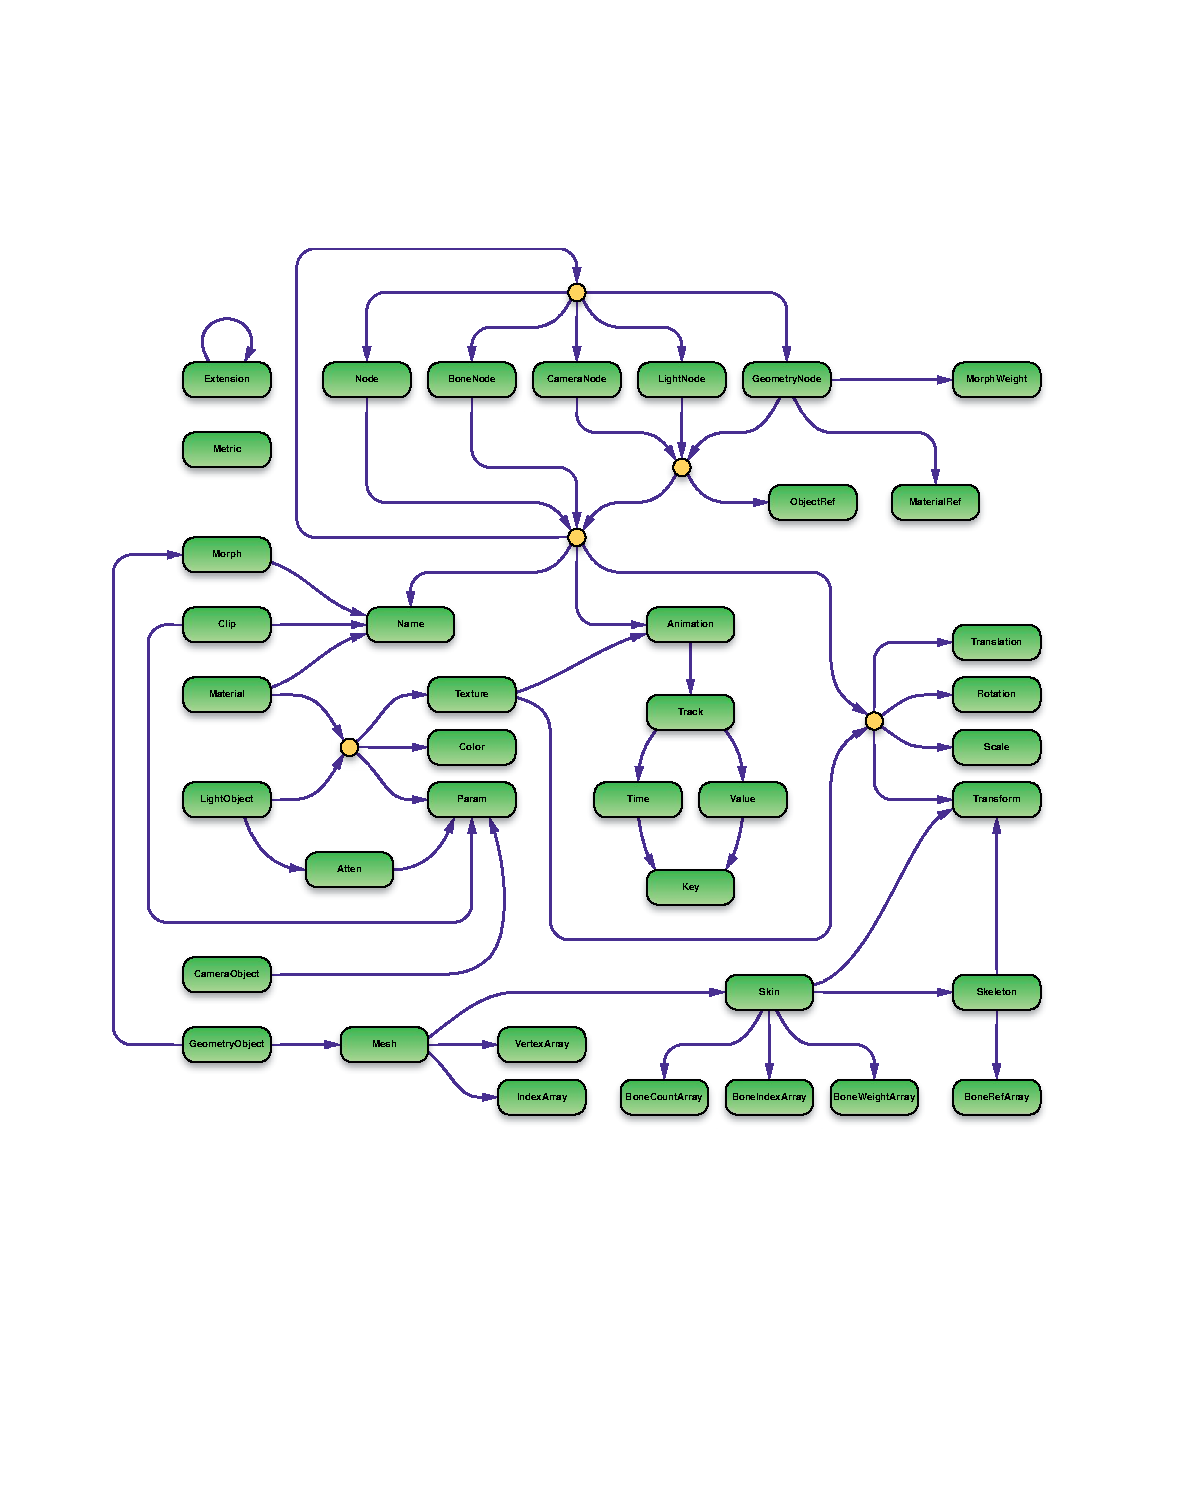
\includegraphics[width=1\textwidth]{images/opengexstruktur}
\caption{OpenGEX Struktur}
\label{fig:opengexstruktur}
\end{figure}